\section{Analysen zum MOT-System}\label{sec:Ergebnisse MOT}
Die Analysen zum MOT-System erfolgen gemäß der Beschreibung in \autoref{sec:Meth MOT}. Es werde die beiden Assoziationsalgorithmen verglichen. Dabei wird die Gesamtperformance unter Verwendung beider Ground Truths gemessen. Anschließend erfolgt die Bewertung der Performance in Abhängigkeit der Verhaltensweise. Die Analyse schließt mit einer Auswertung der Laufzeiten der beiden Assoziationsalgorithmen ab. \par

Das Ziel besteht darin, den besten Algorithmus auszuwählen, die Erfolgsaussichten zu bewerten, aussagekräftige Features aus den Trajektorien generieren zu können und die Beurteilung, wie sich die Laufzeit der Assoziation auf das Modul auswirken kann. \par

Die Ergebnisse der Untersuchungen werden jeweils in einem eigenen Abschnitt vorgestellt und diskutiert. Die Diskussion der Performance des MOT-Systems erfolgt auf Basis der \textit{HOTA}-Metrik. Die \textit{CLEAR MOT} Metrik und die \textit{IDF1} Metrik werden ebenfalls präsentiert. 


\subsection{Vergleich der Assoziationsalgorithmen}

In der Abbildung \ref{fig:ErgebGesamtMOT} ist der Verlauf der \textit{HOTA}-Wertungen über \(\alpha\) zu sehen. Die Tabelle \ref{tab:verglHOTA} zeigt einen Vergleich der Wertungen zu den beiden Algorithmen.

\begin{figure}[htbp]
     \centering
     \begin{subfigure}[b]{0.9\textwidth}
         \centering
         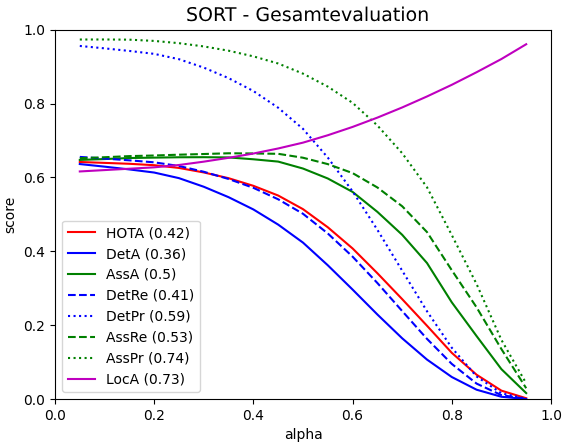
\includegraphics[width=\textwidth, height=11cm]{img/Plots/MOT Evaluation/HOTA SORT Gesamt.png}
         \caption{HOTA Gesamtevaluation des SORT Algorithmus.}
     \end{subfigure}
     \hfill
     \begin{subfigure}[b]{0.9\textwidth}
         \centering
         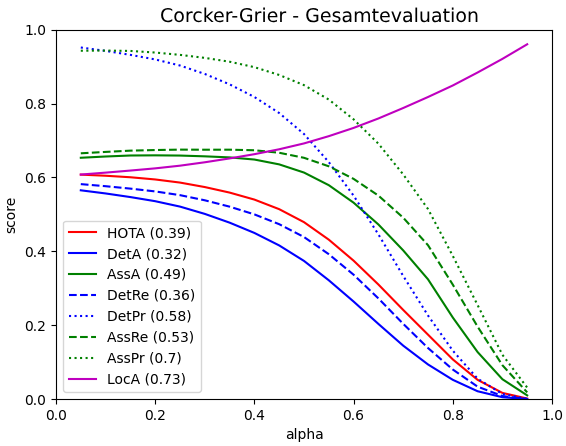
\includegraphics[width=\textwidth, height=11cm]{img/Plots/MOT Evaluation/HOTA CrockGrier Gesamt.png}
         \caption{HOTA Gesamtevaluation des Cocker-Grier Linking Algorithmus.}
     \end{subfigure}
     \caption{Verlauf der \textit{HOTA}-Wertungen der Gesamtperformance der Assoziationsalgorithmen.}
     \label{fig:ErgebGesamtMOT}
\end{figure}

\begin{table}[htbp]
\centering
\caption{Vergleich der Algorithmen mit den HOTA Matriken in \%}
\label{tab:verglHOTA}
\begin{tabular}{
  l
  S[table-format=2.3]
  S[table-format=2.3]
  S[table-format=2.3]
  S[table-format=2.3]
  S[table-format=2.3]
  S[table-format=2.3]
  S[table-format=2.3]
  S[table-format=2.3]
}
\toprule
{Algorithmus} & {HOTA} & {DetA} & {AssA} & {DetRe} & {DetPr} & {AssRe} & {AssPr} & {LocA} \\
\midrule
Cocker-Grier  & 38,797 & 31,857 & 48,526 & 35,691  & 58,362  & 52,639  & 70,188  & 72,863 \\
SORT          & 41,744 & 36,220 & 49,956 & 40,788  & 59,466  & 53,441  & 73,957  & 73,112 \\
\bottomrule
\end{tabular}
\end{table}

Zunächst ist zu bemerken, dass der prinzipielle Verlauf der Performance bei beiden Algorithmen den Erwartungen entspricht. Wie im Beispiel der Abbildung \ref{fig:MPNTrack} zu sehen ist, fallen die Wertungen mit steigendem \(\alpha\) zunehmend, während die Localisation Accuracy steigt. Es ist zu sehen, dass sich die beiden Algorithmen in ihrer Gesamtperformance stark ähneln. Insgesamt schneidet SORT leicht besser ab. Die hohe Ähnlichkeit ist darauf zurückzuführen, dass die Performance von detektionsbasierten Tracking-Systemen stark von den Detektionen beeinflusst wird. Da beide Algorithmen auf den gleichen Detektionen arbeiten, ist die ähnliche Performance nicht verwunderlich. Es ist jedoch eine Bestätigung, dass beide Algorithmen fähig sind, Assoziationen zu tätigen.\dubpar

\textbf{Diskussion der Lokalisationsbewertung}\par
Der SORT Algorithmus verwendet einen Kalman-Filter, welcher die Position der Objekte schätzt, was die Lokalisation beeinflusst. Beim Crocker-Grier Linking Algorithmus wird die Lokalisation nicht beeinflusst. Obwohl der Wert für die Lokalisationsgenauigkeit (LocA) für beide Algorithmen identisch ist, scheint dieser unterschiedliche Umgang keinen Einfluss auf die Performance zu haben.\dubpar

\textbf{Diskussion der Detektionsbewertung}\par
Auch wenn mit den gleichen Detektionen gearbeitet wurde, weisen die Detektionsmetriken Unterschiede auf. Das ist dadurch zu erklären, dass die Algorithmen an unterschiedlichen Stellen und auf unterschiedliche Weisen Detektionen aussortieren. Z.B. verwirft der modifizierte Crocker-Grier Linking Algorithmus Detektionen, wenn sie nicht verifiziert werden können. SORT lässt Detektionen unassoziiert, wenn es keine passende Assoziationen in den folgenden Frames gibt. In diesem Fall wird keine Trajektorie initialisiert. Die niedrige Bewertung des Crocker-Grier Linking Algorithmus deutet darauf hin, dass der Verifizierungsmechanismus die Detektionsqualität negativ beeinflusst. \par

Bei Betrachtung der DetRe und DetPr Wertungen ist zu sehen, dass der Crocker-Grier Linking Algorithmus sowohl mehr falsch positive Fehler macht, als auch mehr falsch negative als SORT. Eine Erklärung für die bessere Detection Precision bei SORT könnte sein, dass das Vorgehen, neue Trajektorien zu initialisieren, dafür sorgt, dass falsch positive Detektionen herausgefiltert werden. Eine andere Erklärung könnte sein, dass der Verifizierungsmechanismus des modifizierten Crocker-Grier Linking Algorithmus dafür sorgt, dass sowohl mehr richtige Detektionen verworfen werden, als auch dafür, dass mehr falsche Detektionen assoziiert werden als bei SORT. \par

\begin{wrapfigure}{l}{0.5\textwidth}
    \begin{center}
        \vspace*{-9mm}
        \begin{subfigure}[b]{0.5\textwidth}
             \centering
             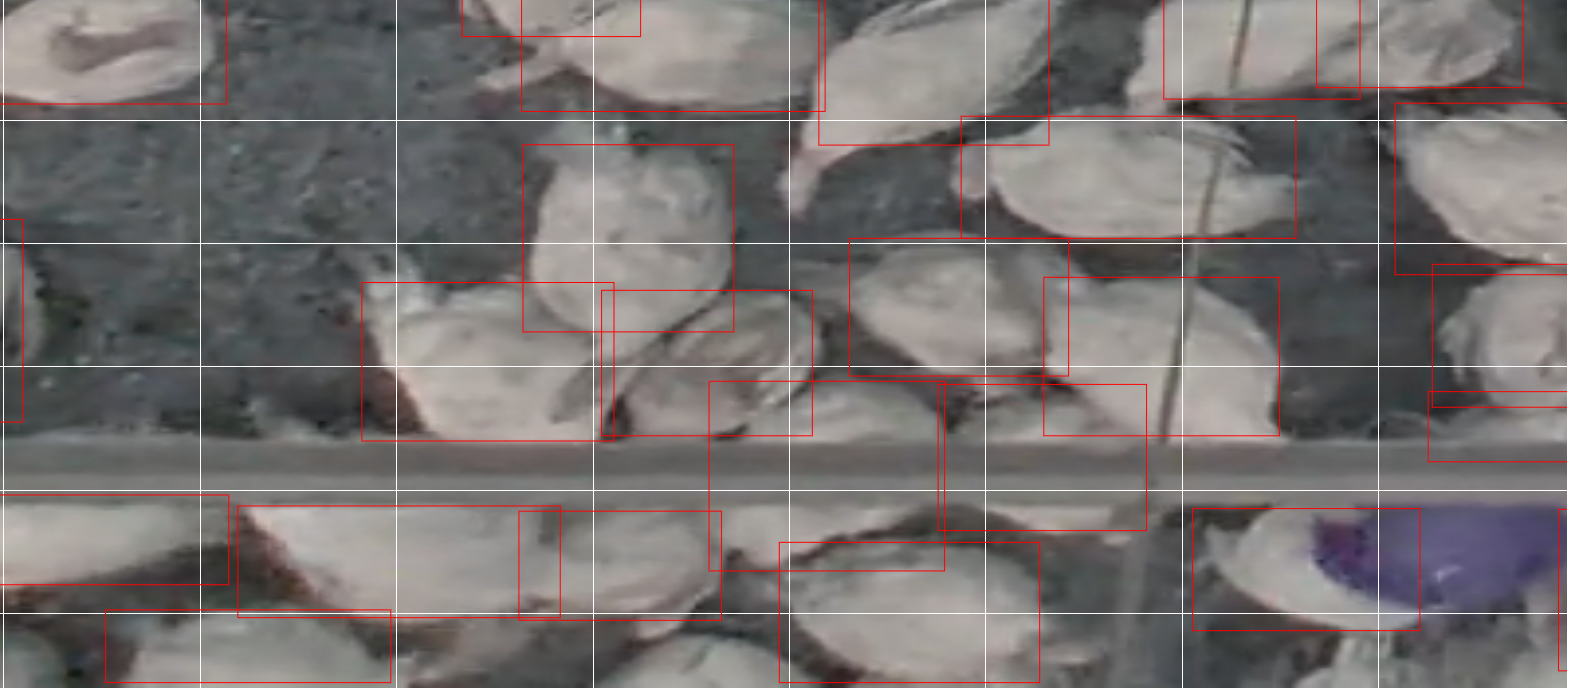
\includegraphics[width=\textwidth]{img/Vergleich GT_Track GT.png}
             \caption{Ground Truth}
         \end{subfigure}
         \hfill
         \begin{subfigure}[b]{0.5\textwidth}
             \centering         
             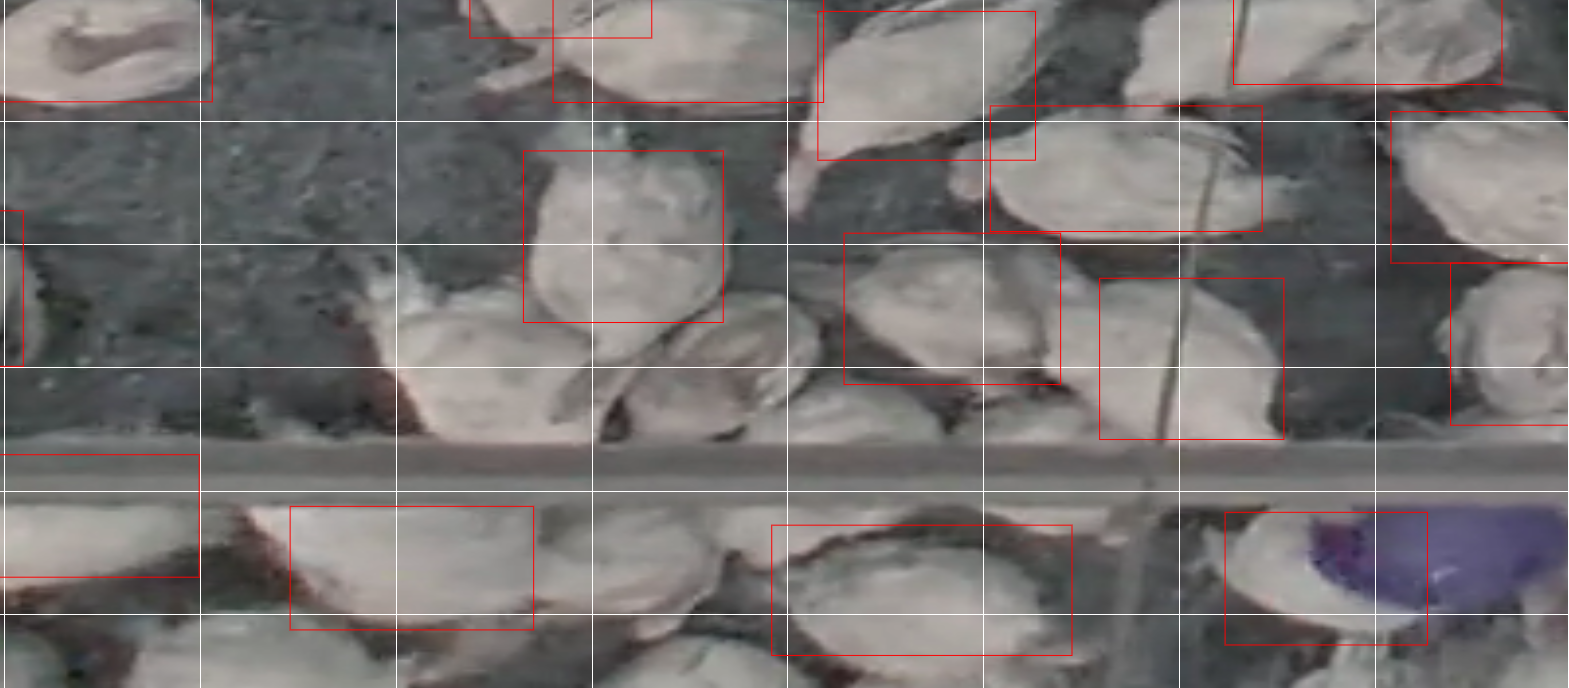
\includegraphics[width=\textwidth]{img/Vergleich GT_Track Tracking.png}
             \caption{Detektionsergebnis}
         \end{subfigure}
        \vspace*{-10mm}
        \caption{Vergleich der Ground Truth und des Detektionsmoduls.}
        \label{fig:GTvsDetsComp}
    \end{center}
\end{wrapfigure}
Bei beiden Algorithmen ist der DetRe Wert niedriger. Das bedeutet, das Detektionsmodul ist anfälliger für falsch negative Detektionen als für falsch positive. Das bedeutet, es werden nicht alle Tiere erkannt. Es ist jedoch davon auszugehen, dass die Mehrdeutigkeiten in der Ground Truth Erstellung sich negativ auf die Bewertung auswirken. Die teilweisen Verdeckungen bei den Futterbahen oder am Randbereich des Kameraausschnitts wurden in der Ground Truth strenger markiert, als es vom Detektionsmodul umgesetzt wird. Dies zeigt sich beim Vergleich der bounding Boxen in der Ground Truth und denen des Detektionsmoduls. In Abbildung \ref{fig:GTvsDetsComp} sind ausgewählte Bildbereiche miteinander verglichen. Sie stammen aus dem gleichen Frame. \par

Somit ist die Bewertung des DetRe-Werts nicht als falsch zu beurteilen, es ist jedoch zu vermuten, dass hier eine Verzerrung entsteht, da das Detektionsmodul vermutlich einen anderen Umgang mit diesen Situationen gelernt hat.\par

Das Ergebnis der Betrachtung der Detektion ist zum Vorteil von SORT. Jedoch sind die Unterschiede nur gering. Da vor allem die Trajektorienqualität entscheidend ist, sind die Assoziationsmetriken ausschlaggebender für die Entscheidung.\dubpar


\textbf{Diskussion der Assoziationsbewertung}\par
Bezogen auf die \textit{HOTA}-Metrik und die DetA-Wertung ist zu sehen, dass das Assoziationsmodul besser abschneidet als das Detektionsmodul. Das ist vorteilhaft, da vor allem die Trajektorienqualität für die Anwendung wichtig ist. Die AssA-Wertung bleibt deutlich länger konstant und wird kaum von \(\alpha\) beeinflusst. \par

Auch hier schneidet SORT besser ab. Während der AssRe-Wert bei beiden Algorithmen gleich ist, unterscheidet sich der AssPr-Wert deutlich. Der  Crocker-Grier Linking Algorithmus ist anfälliger für Merging-Fehler als SORT. Insgesamt ist der AssRe Wert jedoch niedriger als der AssPr-Wert. Das bedeutet, dass beide Algorithmen anfälliger für Fragmentationen als für Merging-Fehler sind.\par

Insgesamt sind die AssRe-Wertung und die AssPr-Wertung als gut zu bewerten. Sie fallen relativ schnell mit steigendem \(\alpha\), jedoch sind sie sehr hoch. Die Fehleranzahl ist also insgesamt niedrig. Das lässt vermuten, dass die Algorithmen Trajektorien generieren können, aus denen sich aussagekräftige Features extrahieren lassen.\dubpar

\textbf{Präsentation der Metriken}

Die Tabelle \ref{tab:MOTgesamtÜbersicht} zeigt eine Übersicht der beiden Algorithmen mit den unterschiedlichen Metriken.

\begin{table}[htbp]
\centering
\caption{Übersicht über die Metriken zu der Beurteilung der Gesamtperformance.}
\label{tab:MOTgesamtÜbersicht}
\begin{tabular}{
  l
  S[table-format=2.3]
  S[table-format=2.3]
  S[table-format=2.3]
  S[table-format=2.3]
  S[table-format=2.3]
}
\toprule
{Algorithmen} & {HOTA} & {MOTA} & {MOTP} & {MODA} & {IDF1} \\
\midrule
Crocker-Grier & 38,797 & 26,278 & 69,156 & 27,103 & 47,870 \\
SORT          & 41,744 & 31,095 & 69,391 & 32,032 & 52,371 \\
\bottomrule
\end{tabular}
\end{table}

\textbf{Fazit}

Die Algorithmen sind in ihrer Performance ähnlich. Insgesamt ist SORT etwas besser. Die Assoziationsqualität verspricht Trajektorien zu genieren, aus denen sich aussagekräftige Features extrahieren lassen. 


\subsection{Analyse der Abhängigkeit der Performance von der Verhaltensweise}
Es sind zwei Ground Truths vorhanden. Eine beinhaltet ein Kampfereignis und die andere einen Kontrollgang. Nach menschlicher Beurteilung besteht der Verdacht, dass die Assoziationsalgorithmen bei höherer Dynamik schlechter performen. Dieser Verdacht wird untersucht. Das Kampfereignis weist deutlich weniger Dynamik auf, als der Kontrollgang.\par

Die Abbildung \ref{fig:SORTHOTAEREIG} zeigt die Verläufe der \textit{HOTA}-Metriken zum SORT Algorithmus, wobei die Bewertung beider Ereignisse dargestellt ist. Abbildung \ref{fig:CROCKHOTAEreig} zeigt dies für die Bewertung des Crocker-Grier Linking Algorithmus. Die Tabelle \ref{tab:HOTAübersEreig} zeigt eine Übersicht über die Ergebnisse.

\begin{figure}[htbp]
     \centering
     \begin{subfigure}[b]{0.9\textwidth}
         \centering
         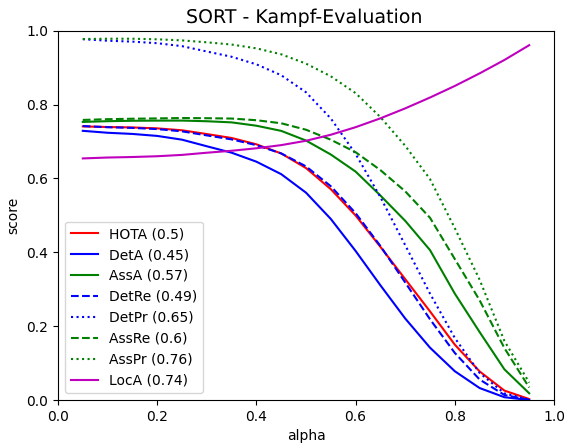
\includegraphics[width=\textwidth, height=11cm]{img/Plots/MOT Evaluation/HOTA SORT Kampf.png}
         \caption{Evaluation mit dem Kampfereignis.}
     \end{subfigure}
     \hfill
     \begin{subfigure}[b]{0.9\textwidth}
         \centering
         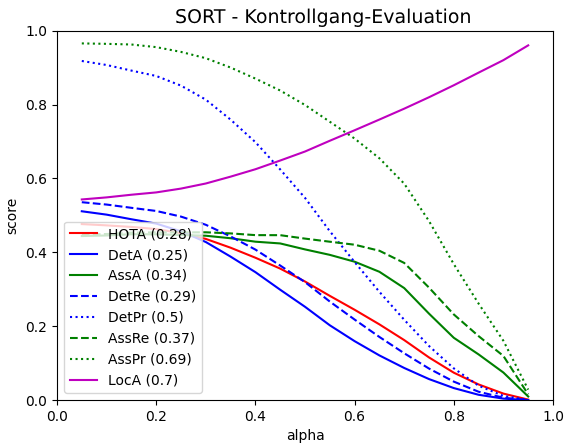
\includegraphics[width=\textwidth, height=11cm]{img/Plots/MOT Evaluation/HOTA SORT Kontrollgang.png}
         \caption{Evaluation mit dem Kontrollgang.}
     \end{subfigure}
     \caption{Evaluation des SORT Algorithmus in Bezug auf die Verhaltensweise.}
     \label{fig:SORTHOTAEREIG}
\end{figure}

\begin{figure}[htbp]
     \centering
     \begin{subfigure}[b]{0.9\textwidth}
         \centering
         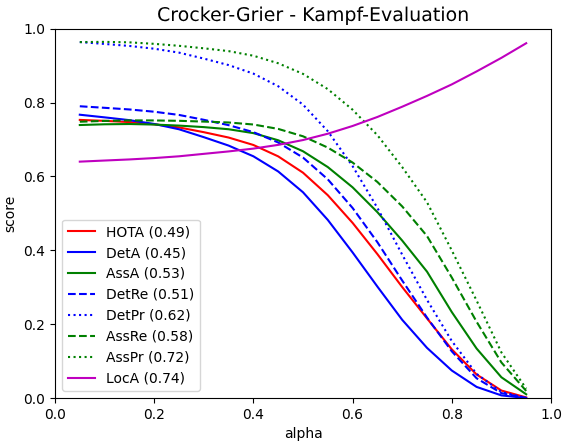
\includegraphics[width=\textwidth, height=11cm]{img/Plots/MOT Evaluation/HOTA CrockGrier Kampf.png}
         \caption{Evaluation mit dem Kampfereignis.}
     \end{subfigure}
     \hfill
     \begin{subfigure}[b]{0.9\textwidth}
         \centering
         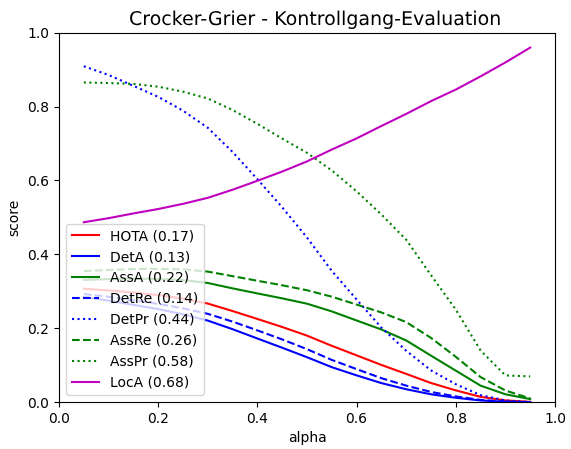
\includegraphics[width=\textwidth, height=11cm]{img/Plots/MOT Evaluation/HOTA CrockGrier Kontrollgang.png}
         \caption{Evaluation mit dem Kontrollgang.}
     \end{subfigure}
     \caption{Evaluation des Crocker-Grier Linking Algorithmus in Bezug auf die Verhaltensweise.}
     \label{fig:CROCKHOTAEreig}
\end{figure}

\begin{table}[htbp]
\centering
\caption{Performance der Algorithmen in Bezug auf das Ereignis.}
\label{tab:HOTAübersEreig}
\begin{tabular}{
  l
  l
  S[table-format=2.2]
  S[table-format=2.2]
  S[table-format=2.2]
  S[table-format=2.2]
  S[table-format=2.2]
  S[table-format=2.2]
  S[table-format=2.2]
  S[table-format=2.2]
}
\toprule
{Algorithmus} & {Ereignis} & {HOTA} & {DetA} & {AssA} & {DetRe} & {DetPr} & {AssRe} & {AssPr} & {LocA} \\
\midrule
SORT          & Kampf      & 49,53 & 44,50 & 56,63 & 49,10  & 64,65  & 60,28  & 75,64  & 74,49 \\
SORT          & Kontrollgang & 28,37 & 25,43 & 33,73 & 29,22  & 50,07  & 36,66  & 69,09  & 70,20 \\
Crocker-Grier & Kampf      & 48,67 & 45,28 & 53,40 & 51,12  & 62,36  & 57,53  & 72,08  & 73,97 \\
Crocker-Grier & Kontrollgang & 28,37 & 25,43 & 33,73 & 29,22  & 50,07  & 36,66  & 69,09  & 70,20 \\
\bottomrule
\end{tabular}
\end{table}

\textbf{Diskussion zum Kampfereignis}\par
Im Vergleich zur Gesamtperformance ist das MOT System besser, wenn es nur mit dem Kampfereignis beurteilt wird. Die grundlegenden Trends bleiben erhalten, wobei SORT in den meisten Metriken besser abschneidet als der Crocker-Grier Linking Algorithmus. Im Vergleich zur Gesamtperformance bleiben die Werte länger konstant, wenn \(\alpha\) steigt. \par

Der Crocker-Grier Linking Algorithmus weist hier einen besseren DetRe-Wert als SORT auf. Das ist damit zu erklären, dass der Verifizierungsmechanismus vermutlich einen Großteil der Trajektorien verifizieren kann. Dadurch bleiben wenige Detektionen ungenutzt. SORT hingegen verwirft offenbar einige echt positive Detektionen, da sie zu keiner Trajektorie initialisiert werden können. Da die restlichen Wertungen des Crocker-Grier Linking Algorithmus jedoch niedriger sind, scheint die erhöhte Menge verifizierter Trajektorien sich nicht positiv auf die Ergebnisse des Systems auszuwirken.\dubpar  


\textbf{Diskussion zum Kontrollgang}\par
Die Performance im Kontrollgang sinkt erheblich. Die Ergebnisse bestätigen den menschlichen Eindruck, dass die Qualität bei erhöhter Dynamik sinkt. Alle Fehlerarten nehmen zu und jede Wertung sinkt im Vergleich zum Kampfereignis. \par

Hier zeigt sich ein deutlicherer Unterschied zwischen den Algorithmen. Der Performanceverlust vom Crocker-Grier Linking Algorithmus ist höher als der von SORT, und das gilt für sämtliche Metriken. Da vor allem die Korrektheit der Trajektorien wichtig ist, um Features zu extrahieren, sind die Assoziationswertungen am relevantesten. SORT ist der Algorithmus, welcher bei höherer Dynamik die richtigeren Trajektorien generiert.\par

Der AssRe-Wert zeigt, dass sich im Kontrollgang Fragmentation häuft. Das kann für die Extraktion von Features problematisch werden. Sind Bewegungen zu stark fragmentiert, spiegeln die Trajektorien eventuell wichtige Merkmale der Bewegung nicht wider. Findet die Fragmentation bspw. immer dann statt, wenn eine explosive Geschwindigkeitserhöhung stattfindet, können die Features, die aus diesen Trajektorien extrahiert werden, die Dynamik des Geschehens nicht abbilden. In der Feature-Auswahl ist zu untersuchen, ob sich mit den extrahierten Features ein Kontrollgang von den anderen Verhaltensweisen unterscheiden lässt. Die Assoziationswertungen des SORT Algorithmus sind jedoch in der Hinsicht vielversprechend, da auch bei hoher Dynamik richtige Trajektorien generiert werden. Ob diese das Geschehen korrekt repräsentierten, muss über die Features untersucht werden.\dubpar


\textbf{Präsentation der Metriken}\par

In Tabelle \ref{tab:MetrikenEregins} sind die unterschiedlichen Metriken im Vergleich dargestellt. Angegeben sind sie zu jedem Ereignis und jedem Algorithmus.

\begin{table}[htbp]
\centering
\caption{Übersicht über die Metriken zu der Bewertung der Ereignisse.}
\label{tab:MetrikenEregins}
\begin{tabular}{
  l
  l
  S[table-format=2.3]
  S[table-format=2.3]
  S[table-format=2.3]
  S[table-format=2.3]
  S[table-format=2.3]
}
\toprule
{Algorithmus} & {Ereignis} & {HOTA} & {MOTA} & {MOTP} & {MODA} & {IDF1} \\
\midrule
SORT          & Kampf      & 49,537 & 50,229 & 70,168 & 50,951 & 65,288 \\
SORT          & Kontrollgang & 28,379 & 4,4885 & 67,252 & 5,722 & 32,415 \\
Crocker-Grier & Kampf      & 48,673 & 48,019 & 69,801 & 48,967 & 63,813 \\
Crocker-Grier & Kontrollgang & 28,379 & 4,4885 & 67,252 & 5,722 & 32,415 \\
\bottomrule
\end{tabular}
\end{table}

\textbf{Fazit}\par
Insgesamt hängt die Performance stark von den Ereignissen und der Dynamik ab. Das Trackingergebnis ist bei hoher Dynamik deutlich schlechter. Gerade bei hoher Dynamik erzeilt der SORT Algorithmus eine deutlich bessere Performance als der Crocker-Grier Linking Algorithmus. Korrekte Trajektorien werden in beiden Ereignissen generiert. In der Feature-Auswahl ist zu überprüfen, ob die extrahierten Features einen Kontrollgang so repräsentieren, dass er sich von den anderen Verhaltensweisen unterscheiden lässt.


\subsection{Vergleich und Auswertung der Laufzeiten}
Die Laufzeiten der beiden Algorithmen sind für unterschiedliche Ereignislängen ermittelt worden. In der Abbildung \ref{fig:plotRunTMOT} sind die Laufzeiten in Abhängigkeit der Ereignisdauer geplottet.

\begin{figure}[htb]
    \centering
    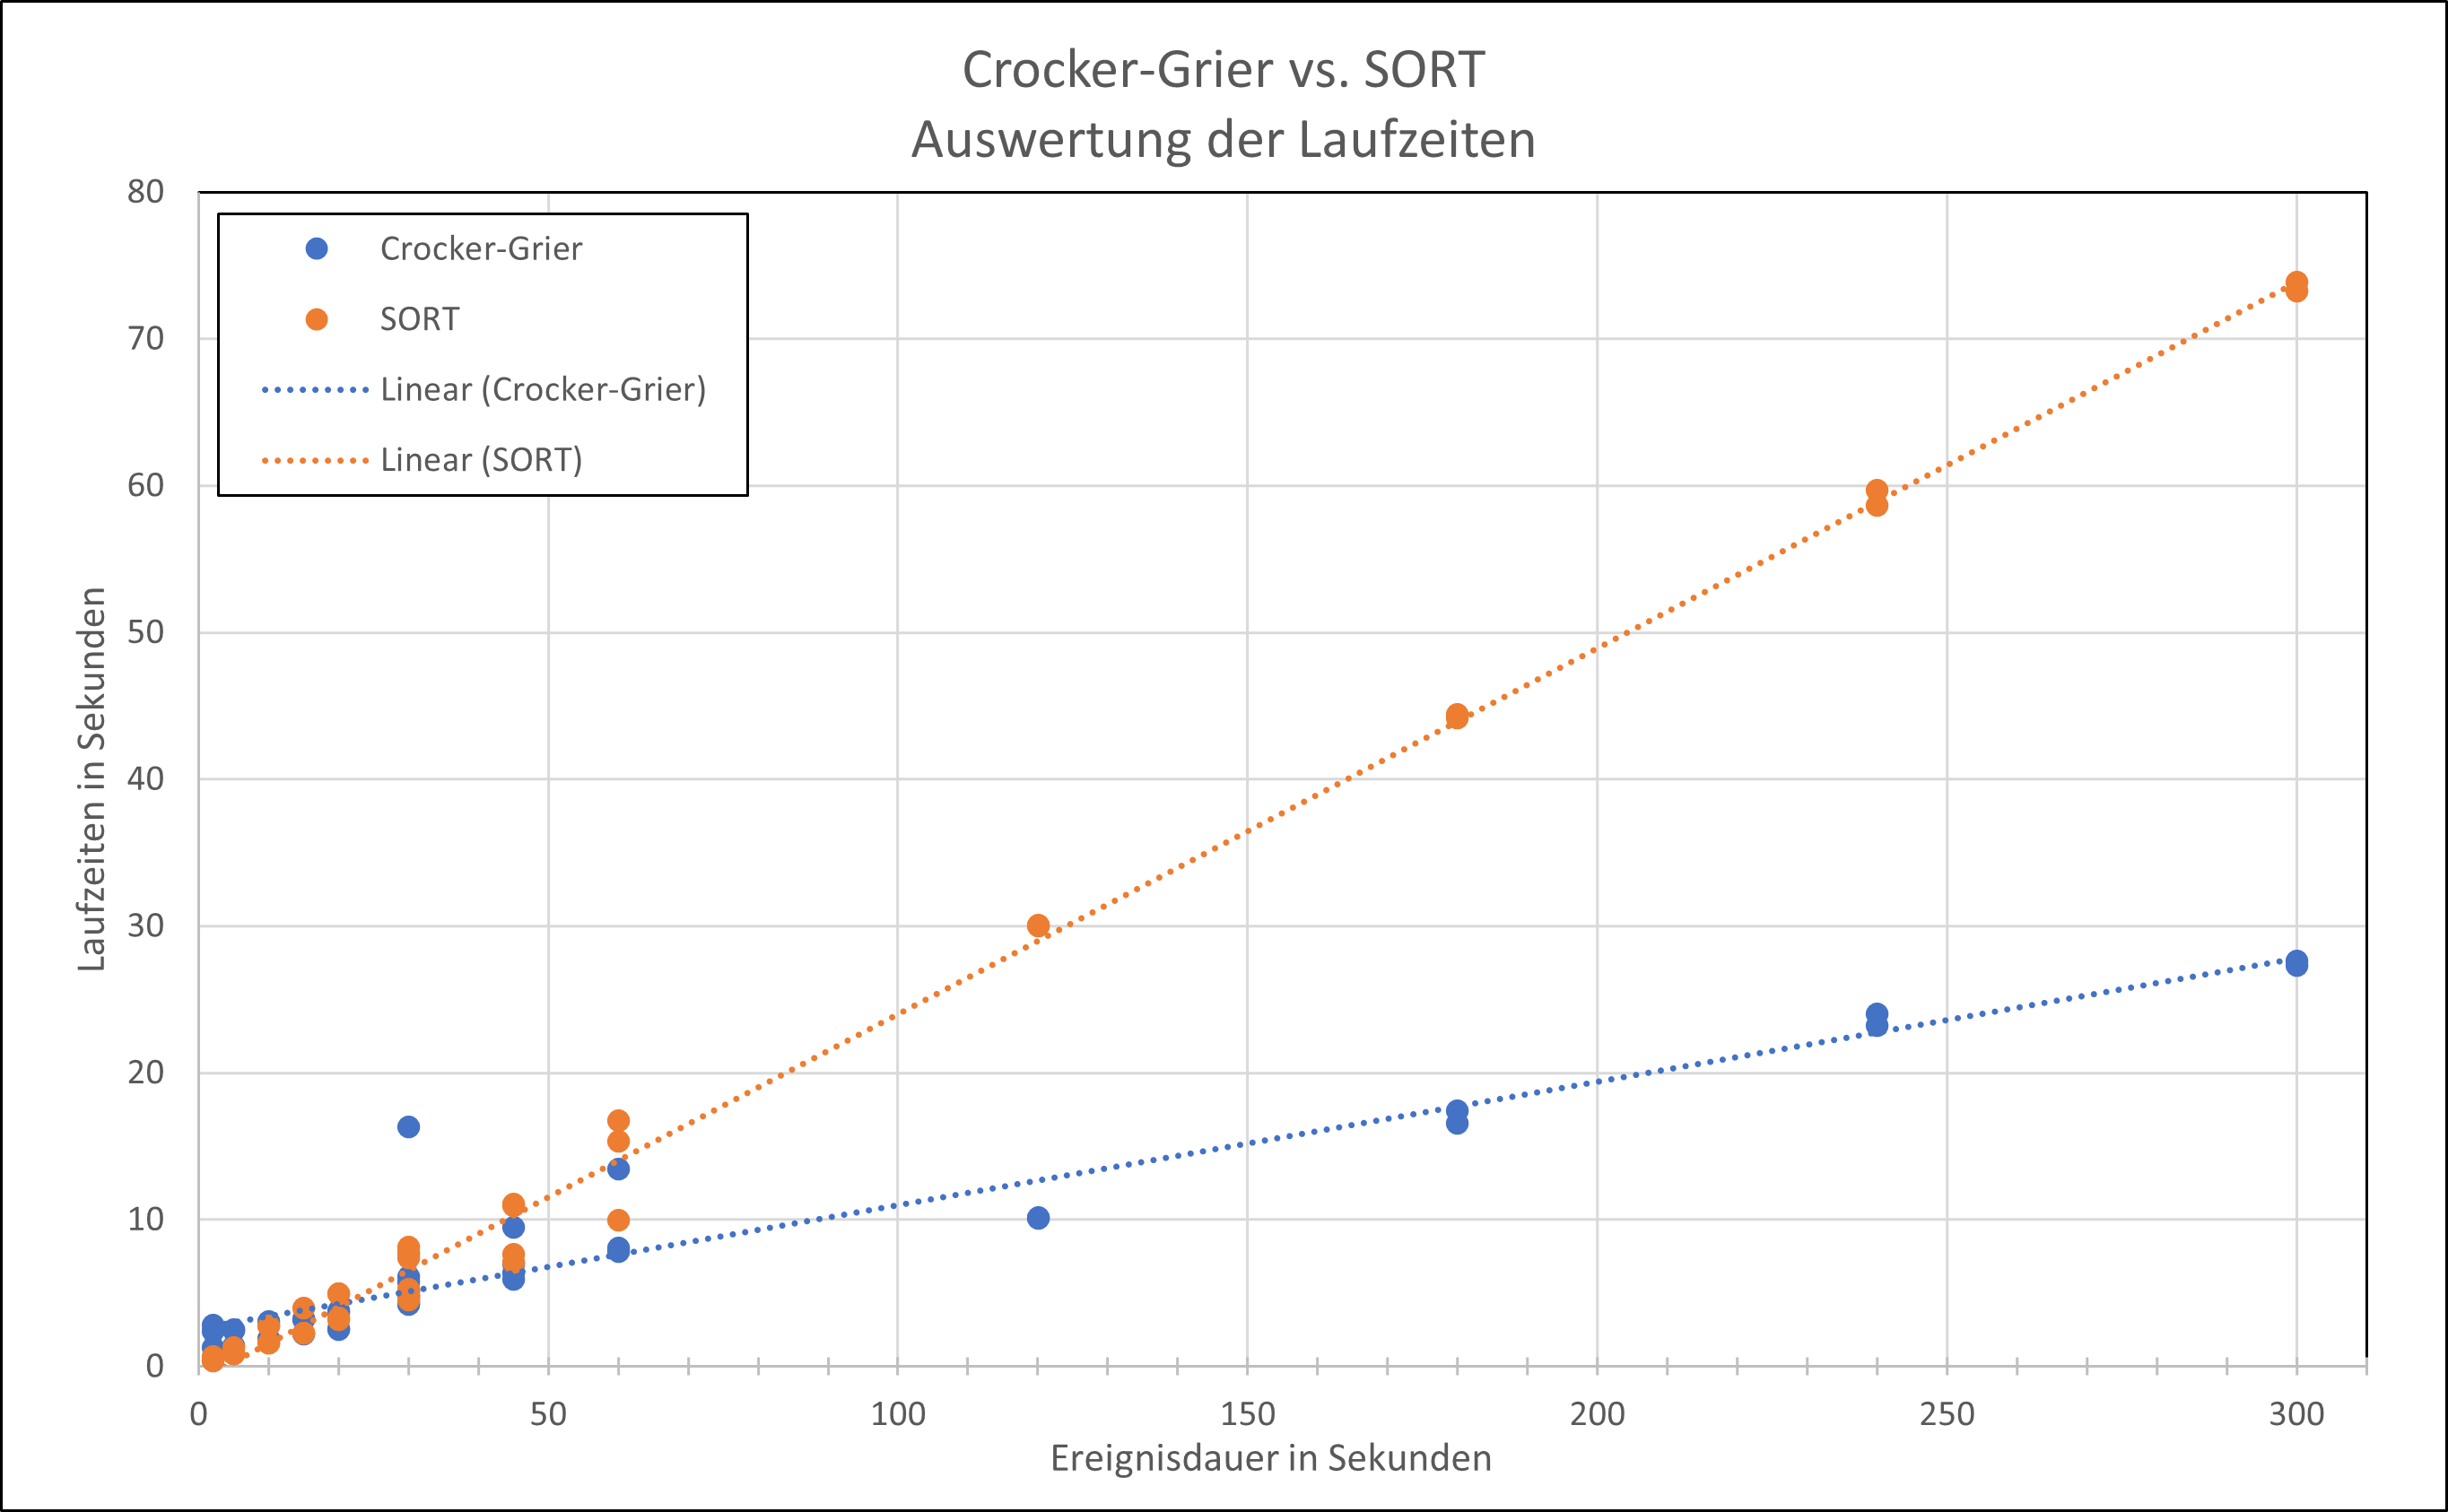
\includegraphics[width=0.9\textwidth]{img/Plots/MOT Evaluation/Assoziationsalgorithmen Laufzeiten.png}  
    \caption{Laufzeiten der Assoziation in Abhängigkeit der Ereignisdauer.}
    \label{fig:plotRunTMOT}
\end{figure}

Es ist zu sehen, dass der Crocker-Grier Linking Algorithmus besser skaliert, jedoch weist er ein klein bisschen mehr Overhead auf. Durch den Overhead ist der zeitliche Vorteil für kleine Ereignislängen von weniger als 30 Sekunden nicht signifikant. Die Trendlinien beider Algorithmen zeigen, dass die Laufzeiten für Ereignisse, die kürzer als 5 Minuten sind, annähernd linear skalieren. Da Beide Trendlinien eine Steigung kleiner eins aufweisen, erfüllen sie die Grundvoraussetzung für die Anwendung im Modul. Andernfalls könnte keine lückenlose Abtastung des Stallgeschehens erfolgen. Nach der Auswahl einer Intervallgröße für die Ereignisse kann über die zeitliche Skalierung der Laufzeit eingeschätzt werden, wie viel Zeit die restliche Verarbeitung in Anspruch nehmen darf, um eine lückenlose Abtastung zu erreichen.  \dubpar

\textbf{Fazit}\par
Die Laufzeit des Crocker-Grier Linking Algorithmus skaliert etwas besser. Für kurze Ereignisse ist der Unterschied jedoch vernachlässigbar. Mit beiden Algorithmen kann eine lückenlose Abtastung des Stallgeschehens erreicht werden.

\subsection{Fazit der Analysen zum MOT System}
Für das Modul wird der SORT Algorithmus verwendet, da er in fast allen Belangen besser performt als der Crocker-Grier Linking Algorithmus. Ausschlaggebend ist die erheblich bessere Performance in hochdynamischen Ereignissen. In solchen Ereignissen besteht die Gefahr, dass die Features, die aus den Trajektorien extrahiert werden, das dynamische Geschehen nicht korrekt repräsentieren. Dies ist zu untersuchen. Insgesamt sind jedoch korrekte Assoziationen in jedem Ereignis zu erwarten. Die Laufzeiten der Algorithmen beeinflussen die Entscheidung zwischen den Algorithmen nicht, da beide die Kriterien in Bezug auf die Laufzeit erfüllen, um im Modul angewendet zu werden.